\section{Types}
\begin{frame}{Types}
  \centering
  
    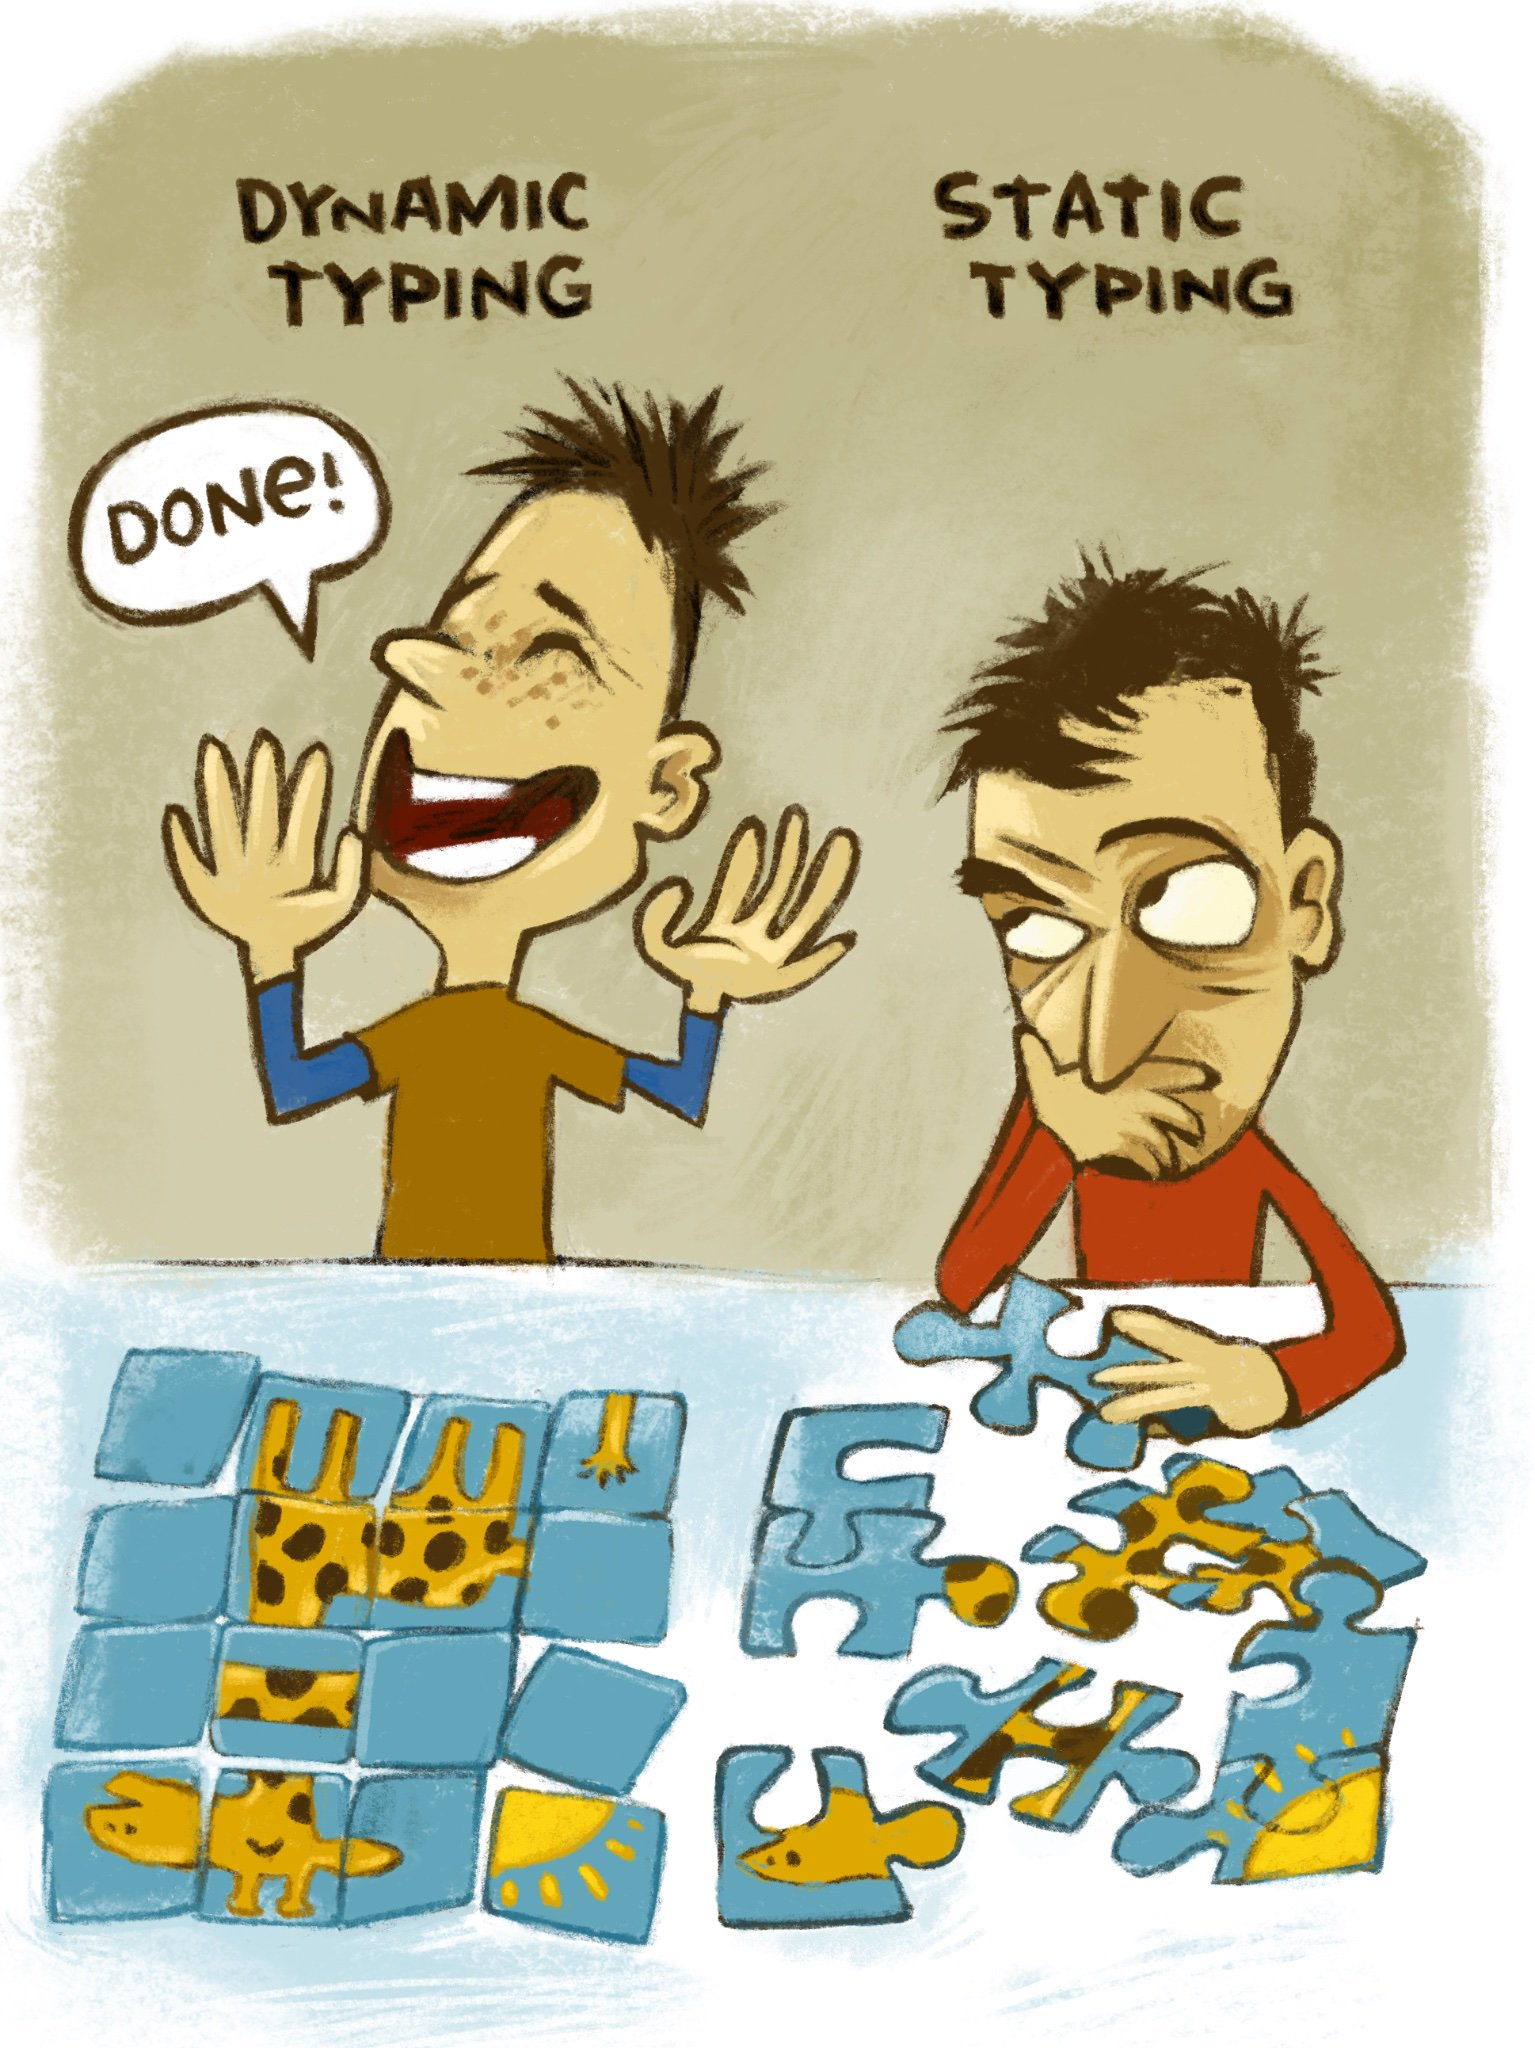
\includegraphics[height=8cm]{typing.png}
\end{frame}

\begin{frame}{Types}{What are Types?}
  \begin{itemize}
  \item Types as Sets
  \item Static
  \item Dynamic
  \end{itemize}
\end{frame}

\begin{frame}{SETS}{Simple Embedded Type System}
  Type system which extends the built-in type system language (Scala, Python, Clojure)

  Modeled after the Common Lisp Type system.

  Supports intersection, union, complement

  Supports deterministic membership check and incomplete subtype check

\end{frame}

\begin{frame}{Genus}{Genus as Alebraic Data Type}
  \begin{itemize}
  \item \code{SAnd} and \code{SOr}, union and intersection
  \item \code{SEmpty} and \code{STop}, empty and universal type
  \item \code{SNot} complement
  \end{itemize}
\end{frame}

\begin{frame}{Genus}{Special Types}
  \begin{itemize}
  \item \code{SAtomic} encapsulates built-in type \code{Class[\_]} \eg, \code{classOf[Int]}.
  \item \code{SMember} and \code{SEql}, explicit types, encapsulates designated values
  \item \code{SSatisfies} encapsulates any predicate: \code{Any => Boolean}.
  \end{itemize}
\end{frame}


\begin{frame}{Subtype}
  The question of type membership is always answerable.

  The question of subtype is sometimes unanswerable. 

  The \code{subtypep} method returns \code{Option[Boolean]} with
  \code{None} meaning that the subtype question could not be answered.
  \begin{itemize}
  \item Unaswerable because impossible \eg \code{SSatisfies}
  \item Unanswerable because code is necessarily incomplete.
  \item Types may be created (by dynamically loaded JVM libraries) after DFA has been constructed.
  \end{itemize}

\end{frame}
